\documentclass[10pt,twocolumn,letterpaper]{article}

\usepackage{cvpr}
\usepackage{times}
\usepackage{epsfig}
\usepackage{graphicx}
\usepackage{amsmath}
\usepackage{amssymb}

% Include other packages here, before hyperref.

% If you comment hyperref and then uncomment it, you should delete
% egpaper.aux before re-running latex.  (Or just hit 'q' on the first latex
% run, let it finish, and you should be clear).
\usepackage[breaklinks=true,bookmarks=false]{hyperref}

\cvprfinalcopy % *** Uncomment this line for the final submission

\def\cvprPaperID{****} % *** Enter the CVPR Paper ID here
\def\httilde{\mbox{\tt\raisebox{-.5ex}{\symbol{126}}}}

% Pages are numbered in submission mode, and unnumbered in camera-ready
%\ifcvprfinal\pagestyle{empty}\fi
\setcounter{page}{1}
\begin{document}

%%%%%%%%% TITLE
\title{Implement of End to End Learning for Self-Driving Cars on Caffe deeplearning framework}

\author{Ruzhuo Wang\\
University of California, Riverside\\
%Institution1 address\\
{\tt\small rwang085@ucr.edu}
% For a paper whose authors are all at the same institution,
% omit the following lines up until the closing ``}''.
% Additional authors and addresses can be added with ``\and'',
% just like the second author.
% To save space, use either the email address or home page, not both
\and
%Second Author\\
%Institution2\\
%First line of institution2 address\\
%{\tt\small secondauthor@i2.org}
}

\maketitle
%\thispagestyle{empty}

%%%%%%%%% ABSTRACT
\begin{abstract}
   In the target paper~\cite{Alpher02}, they trained a convolutional neural network (CNN) to map raw pixels from a single front-facing camera directly to steering commands. Their result is said to be 98\% autonomy value for a typical drive in Monmouth County NJ from their office in Holmdel to Atlantic Highlands.\par
   So I want to find out how they achieve that much high autonomy value, since the target paper do not provide any source code, so I build 3 different but similar architecture of Pilotnet as is mentioned in the targeted paper, and apply two kinds of pre-processing methods for dataset to implement the Pilotnet on Caffe. 
\end{abstract}

%%%%%%%%% BODY TEXT
\section{Introduction}

CNNs have revolutionized pattern recognition. Prior to the widespread adoption of CNNs, most pattern recognition tasks were performed using an initial stage of hand-crafted feature extraction followed by a classifier. The breakthrough of CNNs is that features are learned automatically from training examples. The CNN approach is especially powerful in image recognition tasks because the convolution operation captures the 2D nature of images. Also, by using the convolution kernels to scan an entire image, relatively few parameters need to be learned compared to the total number of operations.\par
End to end (E2E)~\cite{Authors14} deep learning is the idea of instead of engineering a lot of presentations, you can output more complex things.(https://www.quora.com/What-does-end-to-end-mean-in-deep-learning-methods)\par
In this project, I build 3 similar but different architecture of Pilotnet, first one is the same as it is introduced in the target paper, second one is similar with one github project of SullyChen[3](https://github.com/SullyChen/Autopilot-TensorFlow)and the third one is what I build myself. I also apply two pre-processing methods for the original dataset, aiming at improving the performance.


%-------------------------------------------------------------------------
\subsection{Three different network architecture}

I build an architecture that is the same as the target paper introduced, because I think it may have the same performance as is described in the target paper, but the experiment results show that it has the worst performance compared with the architecture I build myself and the architecture of SullyChen's project. \par
After I figure out that the original architecture does not have good performance, I try to modify the architecture and build a new architecture based on the original one by adding some layers, it do increase the train accuracy(the test result that Caffe framework gives out), but it has over-fit problem. \par
In order to furthermore increase the training accuracy and solve over-fit problem, I find out that SullyChen successfully apply Pilotnet on the Tensorflow framework, so I build an architecture the same as he build in Tensorflow project, and it outperforms the other two architectures for train accuracy, but still can not solve the over-fit problem.


\subsection{Two different pre-processing methods for dataset}

I have the original driving dataset that comes from SullyChen's project, in order to improve the training accuracy and solve the over-fit problem, I want to manually extract the feature for the Pilotnet to furthermore increase the training accuracy and solve the over-fit problem, so I apply two pre-processing methods for the original dataset. \par
One pre-processing method is canny edge detector[4]. By applying canny edge detector on the original image, I can extract the curve of the edge in the original image include the road curve. \par
One pre-processing method is image-cropping. By applying this method on the original image, I can extract a smaller image that most of the contains is the road curve. \par




\section{System framework}


%------------------------------------------------------------------------
\subsection{Network architecture}
I build three different but similar Pilotnet architecture as is introduced bellow.
\subsubsection{Original architecture}
The original network consists of 9 layers, including a normalization layer, 5 convolutional layers and 3 fully connected layers. In the target paper, they use strided convolutions in the first three convolutional layers with a $2\times 2$ stride and a $5\times 5$ kernel and a non-strided convolution with a $3\times 3$ kernel size in the last two convolutional layers.

\begin{figure}[h]
	\begin{center}
		
		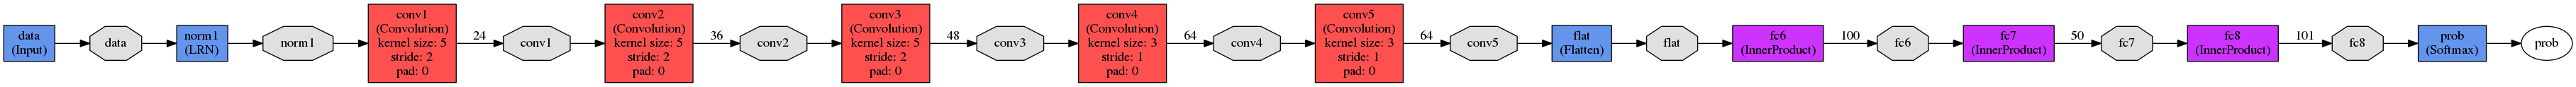
\includegraphics[width=0.8\linewidth]{pilotnet_deploy_original.png}
	\end{center}
	\caption{Original architecture}
	\label{fig:long1}
	\label{fig:onecol1}
\end{figure}

\subsubsection{My architecture}


My network consists of 20 layers, compared with original architecture, I delete one normalization layer, add 7 relu layers, add two new normalization layers and two dropout layers.



\begin{figure}[h]
	\begin{center}
		
		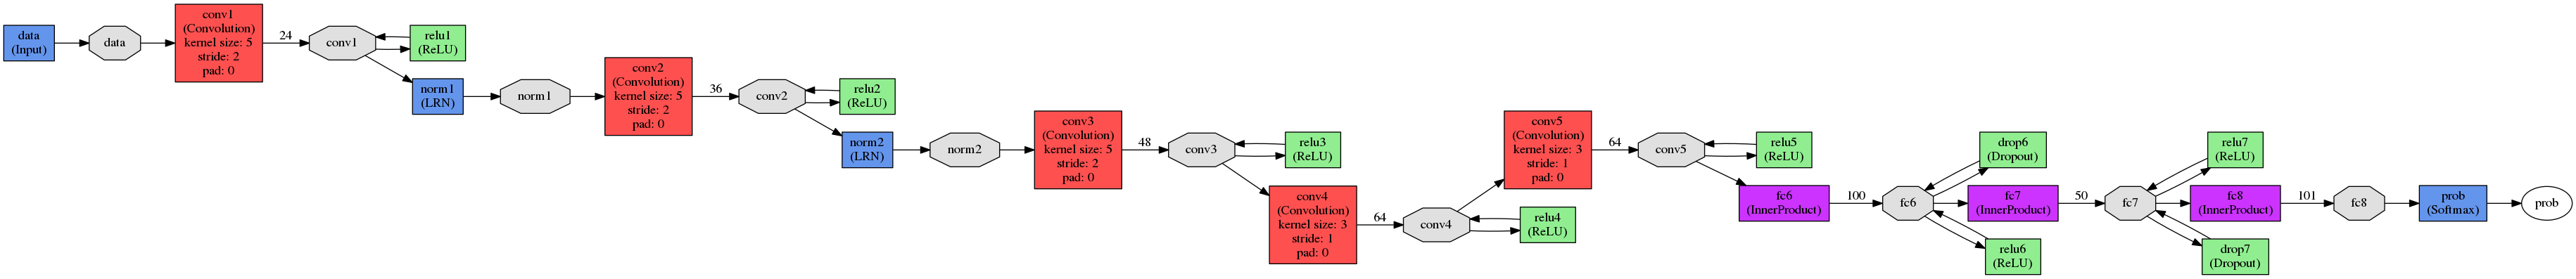
\includegraphics[width=0.8\linewidth]{pilotnet_deploy_my.png}
	\end{center}
	\caption{my architecture}
	\label{fig:long2}
	\label{fig:onecol2}
\end{figure}


\subsubsection{SullyChen's architecture}


SullyChen's network consists of 17 layers, compared with original architecture, SullyChen delete one normalization layer, add 7 relu layers, add two dropout layers.



\begin{figure}[h]
	\begin{center}
		
		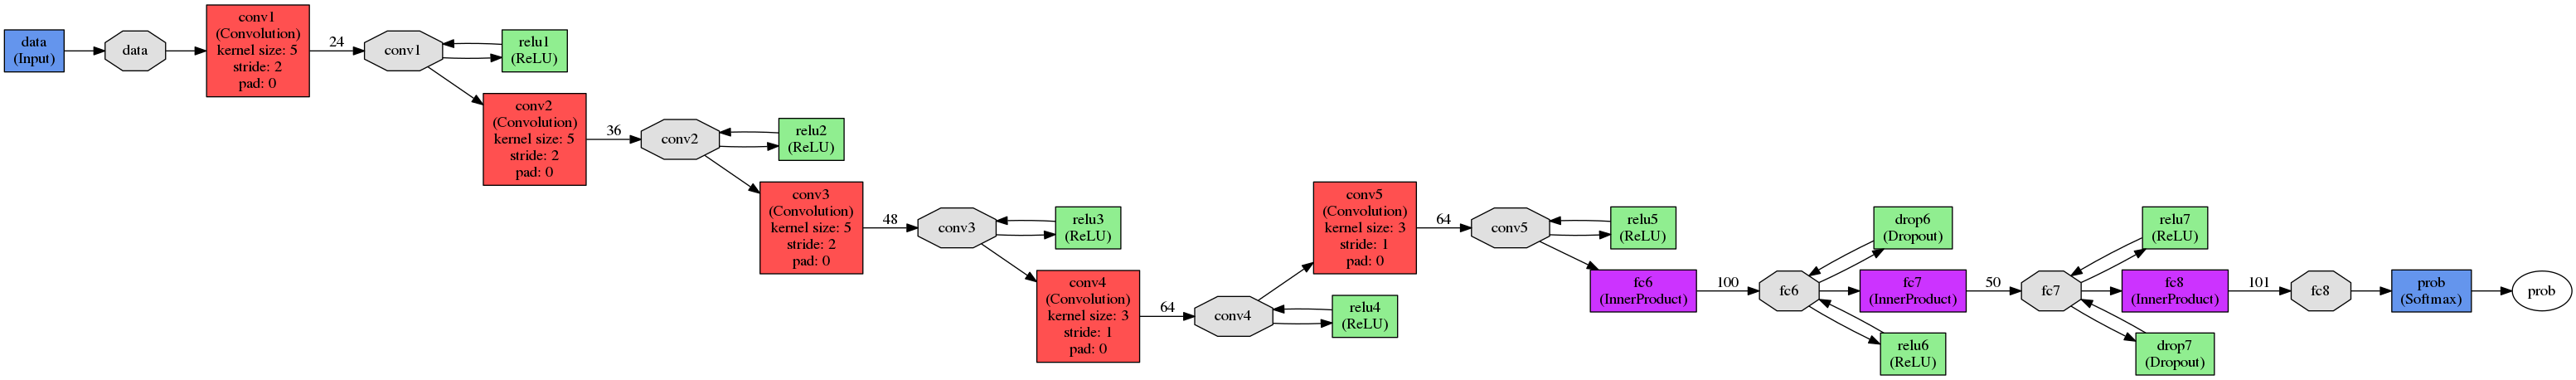
\includegraphics[width=0.8\linewidth]{pilotnet_deploy_s.png}
	\end{center}
	\caption{my architecture}
	\label{fig:long3}
	\label{fig:onecol3}
\end{figure}
%-------------------------------------------------------------------------
\subsection{Important preparation before training}

\subsubsection{The preparation of training and testing dataset}
I write a python script(datasetreader.py) to divide the dataset into two parts, 7/8 of the driving dataset has been treat as training dataset, the other 1/8 of the driving dataset has been treat as test dataset, the driving dataset is consist of 45568 images that captured from a front camera on a driving car. I download this dataset from SullyChen's github repository.

%-------------------------------------------------------------------------
\subsubsection{The label method for dataset}


\begin{figure}[h]
	\begin{center}
		
		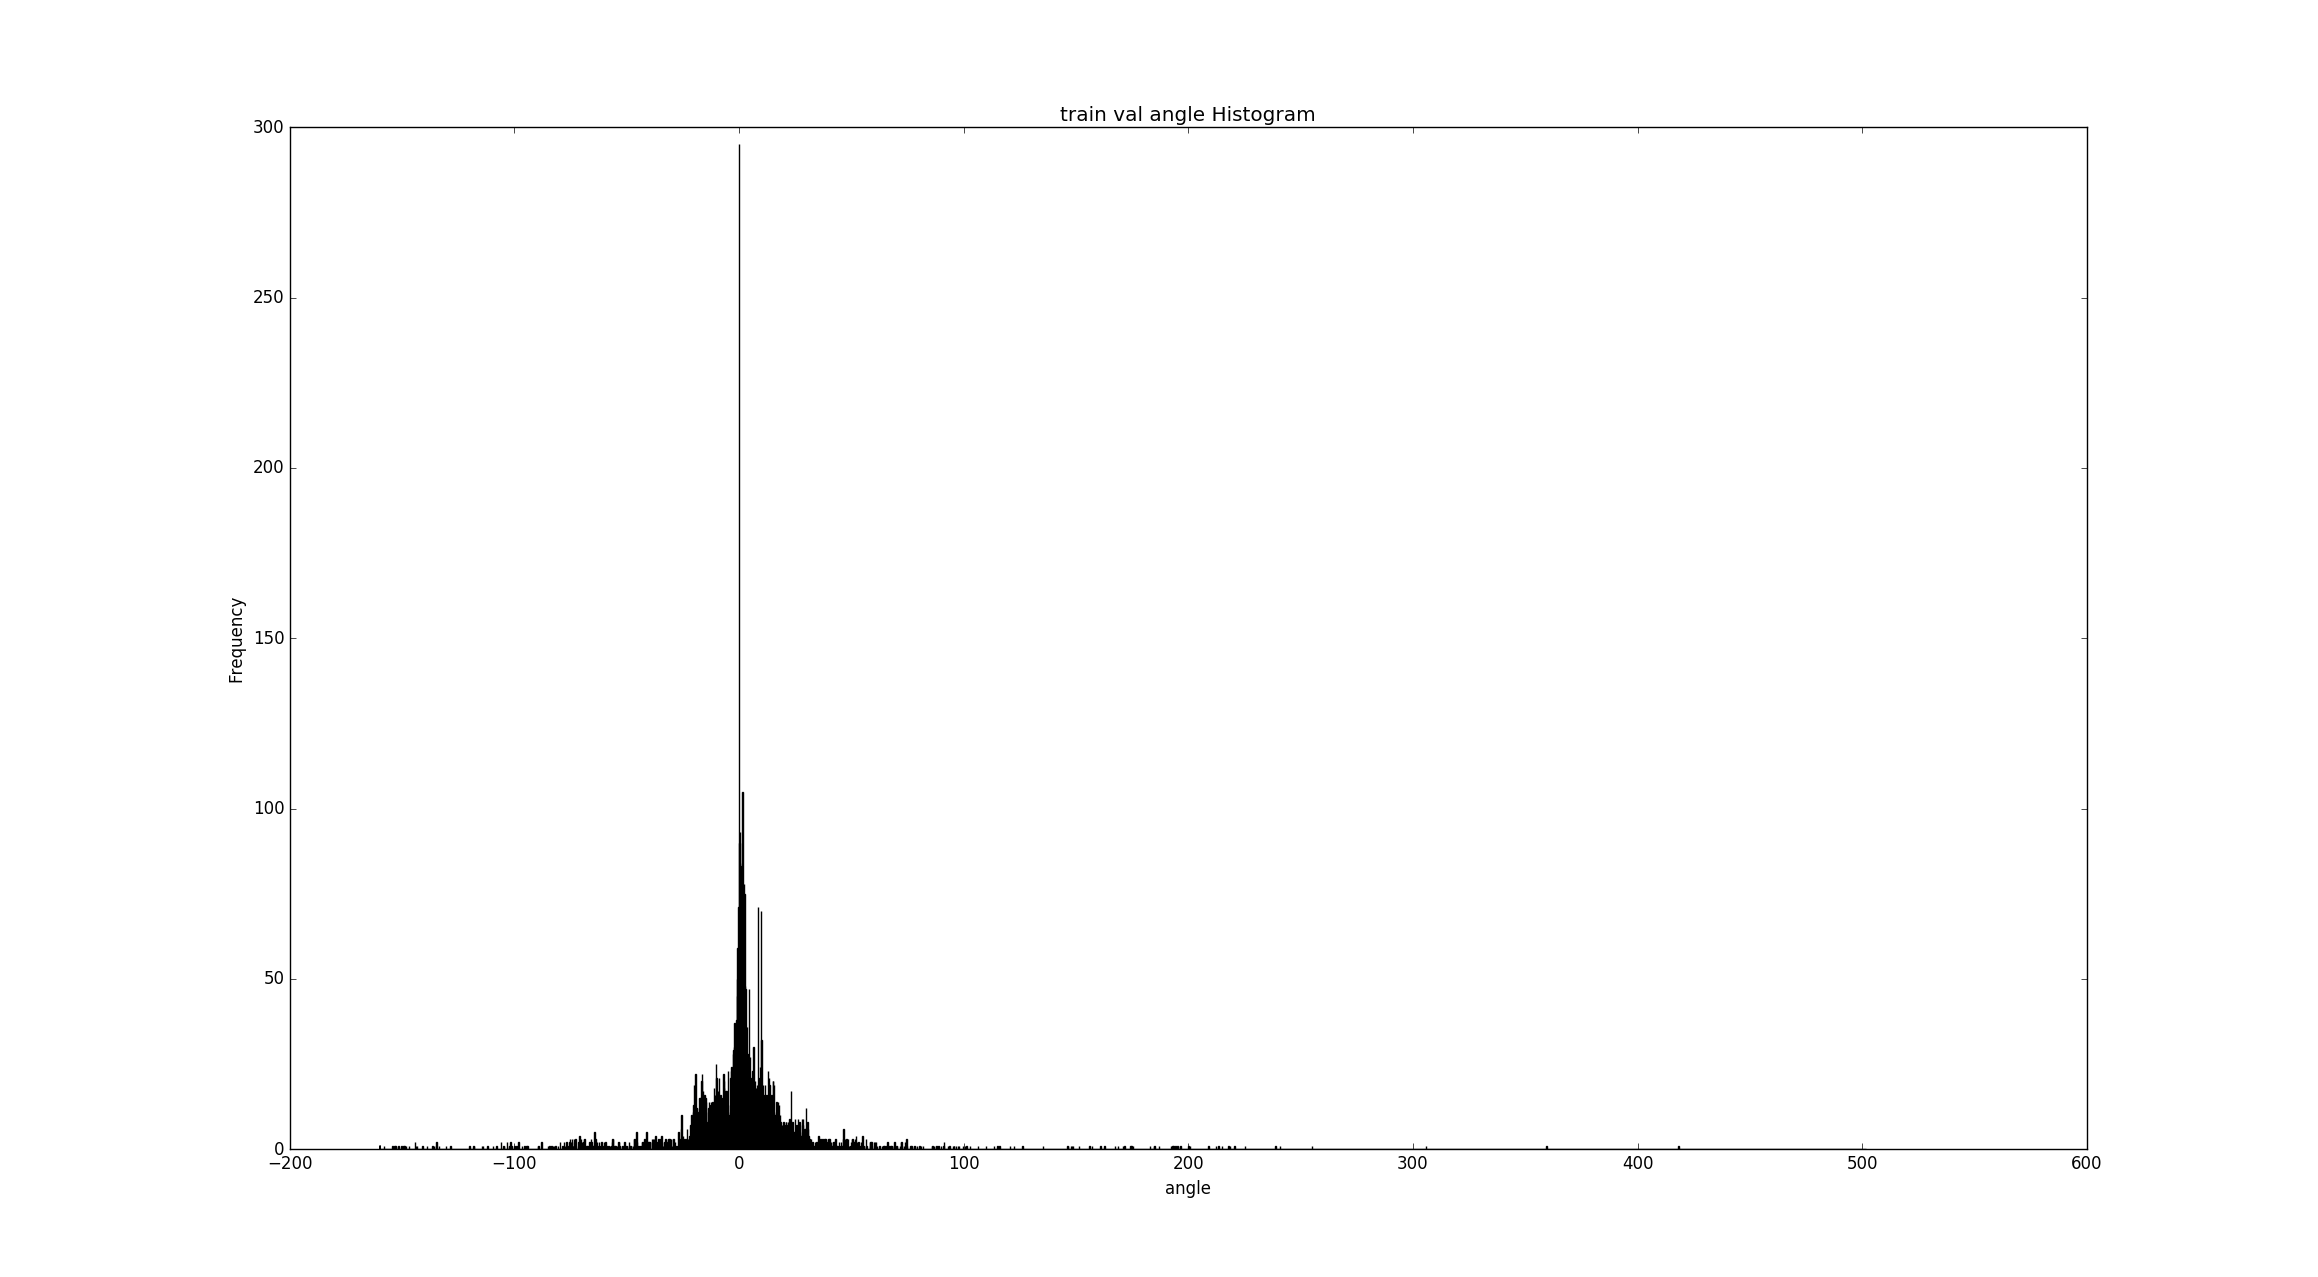
\includegraphics[width=0.8\linewidth]{steering_angle.png}
	\end{center}
	\caption{Steering angle distribution}
	\label{fig:long4}
	\label{fig:onecol4}
\end{figure}

\begin{figure}[h]
	\begin{center}
		
		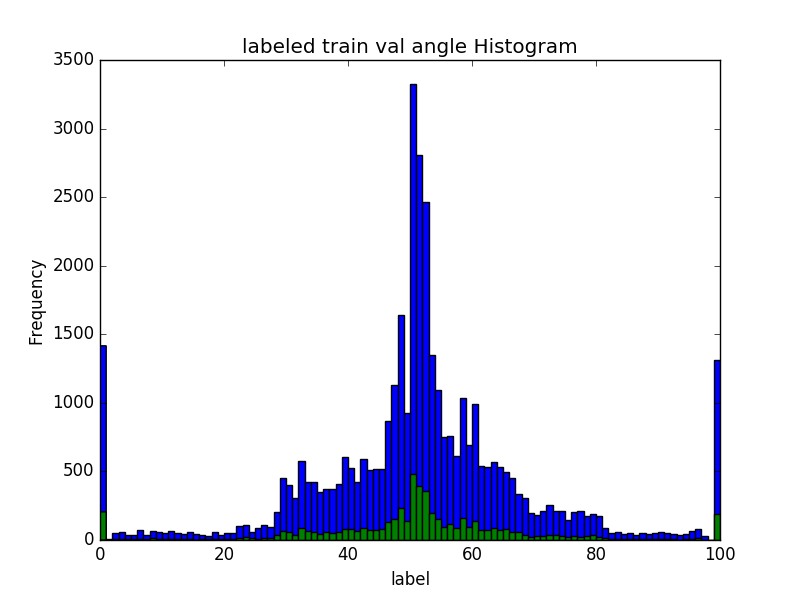
\includegraphics[width=0.8\linewidth]{label_angle.png}
	\end{center}
	\caption{Labeled angle distribution}
	\label{fig:long5}
	\label{fig:onecol5}
\end{figure}


Because the Pilotnet is an end to end network, so it require labeled dataset as training and testing dataset, and for Caffe deeplearning frame work, it require positive integer as label, so I write a python script(label.py) to transfer the steering angle from float number into 0 to 100 labels, because the steering angle is like a Gaussian distribution, the majority steering angle is around 0, so I map the steering angle with the value within -140 to 140 into 1 to 98, the steering angle with the value less than -140 into 0, the steering angle with the value between within 140 to 200 into 99, the steering angle with the value bigger than 200 into 100.





%-------------------------------------------------------------------------
\section{Experiment}

\subsection{For different network architectures}


\begin{figure}[h]
	\begin{center}
		
		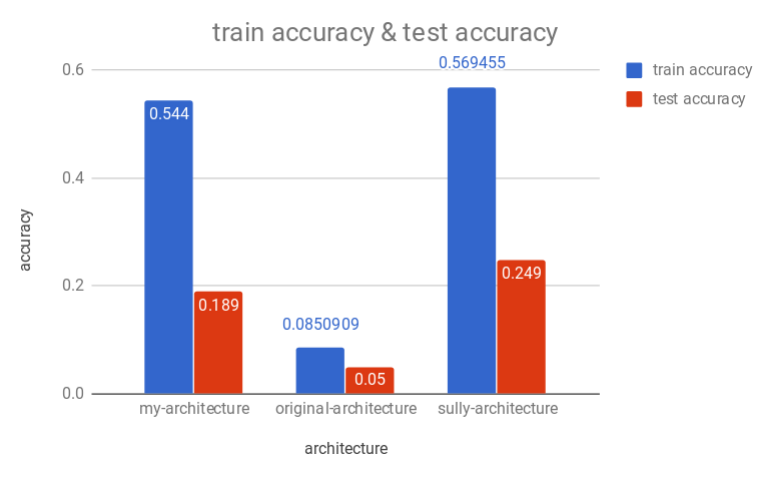
\includegraphics[width=0.8\linewidth]{accuracy.png}
	\end{center}
	\caption{The accuracy performance}
	\label{fig:long7}
	\label{fig:onecol7}
\end{figure}


I train the three different network on the same training dataset, and focus on the train accuracy and test accuracy. The accuracy result in Figure6 shows that SullyChen's architecture outperforms other two. The data in Figure6 is the accuracy performance for three different architectures trained and tested on the original dataset for 10000 iterations.






%------------------------------------------------------------------------


\subsection{Over-fit experiment}



In Figure 7, I can tell that, when iterations increase, the train loss decrease, the training accuracy increase, the train loss here is the test result that Caffe framework give me, but when I test the pre-trained model myself using a python script(prediction.py), and compute the test accuracy, mean error and matched label number using a python script(compute\_prediction\_accuracy.py), the result tell me there exit over-fit problem for pre-trained model.

\begin{figure}[h]
	\begin{center}
		
		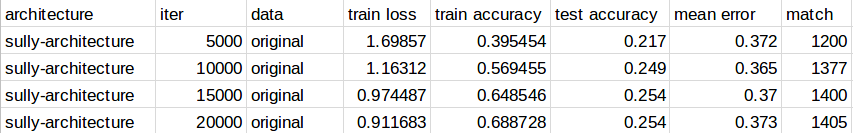
\includegraphics[width=0.8\linewidth]{overfit.png}
	\end{center}
	\caption{Steering angle distribution}
	\label{fig:long6}
	\label{fig:onecol6}
\end{figure}


Also in figure 8, I can tell that, most of the matched label are on the left side, right side and center, mainly because training dataset are located at those positions. The data in figure8 is the prediction result for SullyChen's architecture of 20000 iterations trained and test on the original dataset.

\begin{figure}[h]
	\begin{center}
		
		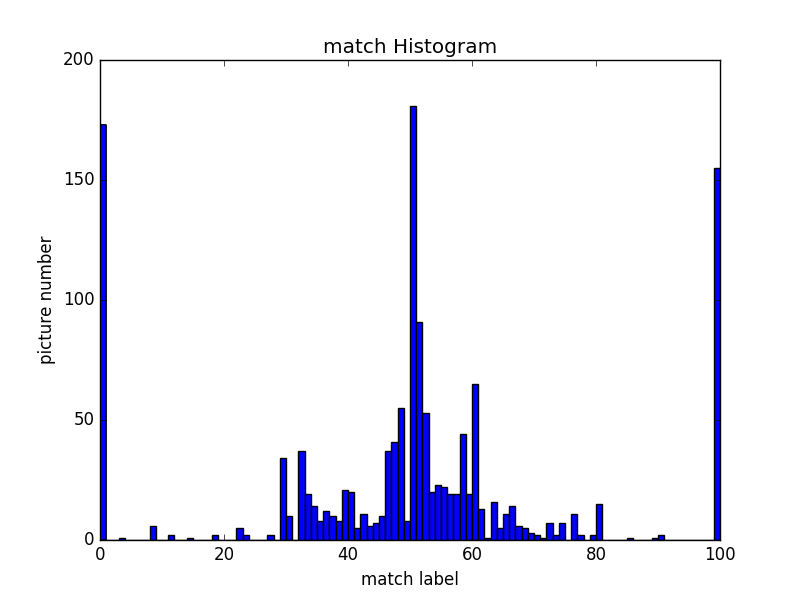
\includegraphics[width=0.8\linewidth]{mh9.png}
	\end{center}
	\caption{Matched label distribution}
	\label{fig:long8}
	\label{fig:onecol8}
\end{figure}


\subsection{For different dataset preprocessing methods}



{\small
\bibliographystyle{ieee}
\bibliography{egbib}
}






\end{document}
